\chapter{Resultados}

Neste capítulo serão apresentados os resultados obtidos nos testes de carga e busca dos dados. Os testes foram realizados em quatro configurações de \emph{cluster}, com uma, duas, quatro e seis máquinas, a fim de se analisar a melhora do desempenho de um banco de dados não relacional ao se aumentar o número de nós. Além disso, em cada configuração de \emph{cluster}, foram realizados três testes com diferentes volumes de dados. 

Em cada configuração de teste foram realizadas dez repetições, tanto na inserção quanto na busca, a fim de garantir resultados mais consistentes. 

\section{Carga de dados}
A carga de dados foi realizada a partir da leitura dos arquivos \emph{.csv} de dados do Bolsa Família, com seleção das colunas a serem utilizadas e tratamento de alguns campos.
Os dados foram carregados a partir de uma única máquina utilizando aplicação desenvolvida, sendo o \emph{Cassandra} responsável pela distribuição dos mesmos dentro do \emph{cluster} . Foi feita também uma comparação entre os tempos observados em cada uma das configurações utilizadas. Esta seção descreve em detalhes essas operações.

\subsection{Preparação e carga}
Foi desenvolvida uma aplicação Java responsável por toda a operação da inserção dos dados com uso do \emph{driver} da \emph{Datastax}. A aplicação realiza a leitura dos dados à partir dos arquivos .csv e utiliza apenas os campos que serão utilizados na família de colunas do banco de dados: \textbf{UF, Código SIAFI Município, Nome Município, NIS Favorecido, Nome Favorecido, Fonte-Finalidade, Valor Parcela, Mês Competência}. Além disso, os campos Valor Parcela e Mês Competência tiveram seus valores tratados para a correta inserção no banco.

No campo Valor Parcela foi necessária a remoção do separador de milhares(',') para se adequar ao tipo \emph{double} do Cassandra. Para o campo Mês Competência, que originalmente segue o padrão MM/AAAA, não é suportado pelo Cassandra, foi necessária a inclusão de um dia para a correta utilização do tipo \emph{timestamp}, sendo então armazenado no formato DD/MM/AAAA.

A carga foi realizada com três volumes de dados, correspondentes a seis meses, um ano e dois anos de informações do Bolsa Família, a fim de se analisar o desempenho do banco com diferentes números de nós ao se aumentar o volume de dados. A tabela~\ref{tab:volume} apresenta o tamanho total dos dados inseridos em cada uma dessas cargas.

\begin{table}[]
	\centering
	\caption{Volume da dados}
	\label{tab:volume}
	\begin{tabular}{ll}
		\textbf{Carga} & \textbf{Tamanho} \\ \hline
		6 meses        &  2,94 GB             \\ \hline
		1 ano          &  5,88 GB             \\ \hline
		2 anos         &  11,79 GB             \\ \hline
	\end{tabular}
\end{table}

A inserção foi realiza de maneira assíncrona com uso de funções disponibilizadas pelo \emph{driver} da \emph{Datastax}. A \emph{query} em formato CQL~\ref{lst:cql_insert} é montada e tem seus parâmetros substituidos, e então ela é executada com o comando \emph{executeAsync} da classe \emph{Session} do \emph{driver}. São realizadas operações em seis \emph{threads} simultâneas, valor que apresentou o melhor resultado nos testes realizados.

Os testes foram repetidos para as configurações de \emph{cluster} com duas, quatro e seis máquinas, com objetivo de analisar uma possível melhora no desempenho em \emph{clusters} maiores.

\begin{lstlisting}[caption={Código CQL para inserção},label={lst:cql_insert},language=SQL]
INSERT INTO bolsa_familia.dados (uf, cod_municipio, nome_municipio, nis_favorecido, nome_favorecido, fonte, valor, periodo) VALUES (?, ?, ?, ?, ?, ?, ?, ?)
\end{lstlisting}

A Tabela~\ref{tb_insert} apresenta os tempos obtidos na inserção dos dados nos diferentes ambientes e volumes de dados. O gráfico~\ref{fig:graph_insert} apresenta os mesmo dados para melhor visualização.


\begin{table}[]
	\centering
	\caption{Inserção}
	\label{tb_insert}
	\begin{tabular}{lllll}
		\textbf{Tamanho}	& \textbf{1 nó} & \textbf{2 nós} & \textbf{4 nós} & \textbf{6 nós} \\ \hline
		\textbf{6 meses}    & 25m37s        & 28m02s         & 27m15s         & 26m29s         \\ \hline
		\textbf{1 ano}      & 51m19s        & 55m25s         & 54m16s         & 52m22s         \\ \hline
		\textbf{2 anos}     & 01h44m53s     & 01h59m17s      & 01h46m57s      & 01h43m56s      \\ \hline
	\end{tabular}
\end{table}

\subsection{Comparação dos ambientes}

Pelos resultados obtidos é possível observar uma melhora no tempo de inserção com uso de mais máquinas no \emph{cluster}, com exceção do caso de apenas um nó, fato que provavelmente ocorre devido às limitações do ambiente de testes utilizado, que se utiliza da rede interna da UnB para a transferência de dados entre as máquinas. Mesmo assim, é possível observar que ao se aumentar o volume dos dados, um aumento do número de máquinas apresenta uma tendência de melhora nos tempos obtidos.

Para o teste com dados de 6 meses, a melhoria média ao se aumentar o número de máquinas foi de \textbf{2,8\%}, para 1 ano foi de \textbf{2,78\%}, e para 2 anos foi de \textbf{6,58\%}, desconsiderando-se os resultados com uma máquina.

\begin{figure}[!htb]
	\centering
	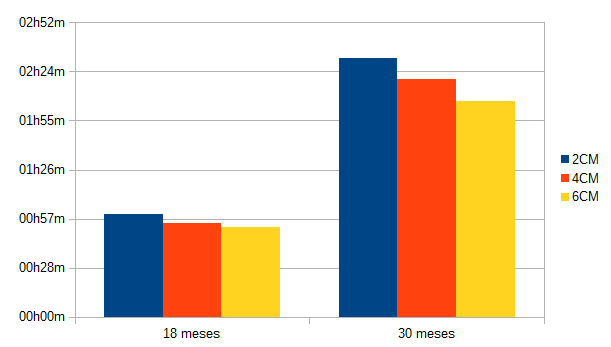
\includegraphics[width=1\textwidth]{figuras/graphinsert.png}
	\caption{Inserção de dados}
	\label{fig:graph_insert}
\end{figure}

\section{Extração de dados}
Após cada inserção dos dados, nas quatro configurações de \emph{cluster} (uma, duas, quatro e seis máquinas), e com os três volumes diferentes de dados, foram realizadas consultas para verificar o desempenho de um banco de dados Cassandra ao se realizar extração de dados.

\subsection{Consultas}
Assim como para a carga de dados, foi desenvolvida uma aplicação Java para a realização das consultas no banco de dados, com uso do \emph{driver} da \emph{Datastax}. Cada teste de consulta envolveu a execução de trinta \emph{Selects} no banco, sendo que cada um realiza uma consulta com uso da linguagem CQL a um registro específico, selecionado de forma aleatória. Essa consulta, exemplificada em \ref{lst:cql_select}, contém toda a totalidade da chave primária da tabela, requisito imposto pelo banco de dados Cassandra. Cada teste foi repetido dez vezes a fim de se obter uma média dos resultados encontrados.

\begin{lstlisting}[caption={Consulta CQL},label={lst:cql_select},language=SQL]
SELECT * FROM dados WHERE uf = 'MS' AND periodo = '2014-07-01' AND valor = 147.00 AND nis_favorecido = 00020915229557
\end{lstlisting}

A tabela \ref{tab:select_busca} apresenta os tempos obtidos na consulta de registros nos diferentes ambientes e volumes de dados testados. O gráfico \ref{fig:graph_select_busca} apresenta os mesmos dados para melhor visualização.

\subsection{Comparação dos ambientes}
Analisando-se os resultados obtido é possível notar uma significativa melhoria nos tempos ao se adicionar mais máquinas no \emph{cluster}. Ao contrário da inserção, a extração de dados apresentou uma melhora média de 70,14\% ao se aumentar o número de máquinas de um para dois. Considerando-se todas as diferenças de tamanho de \emph{cluster} e de volumes de dados, obtemos uma melhora média de \textbf{30,52\%}.~\ref{tab:melhora_select}

\begin{table}[]
	\centering
	\caption{Busca de dados}
	\label{tab:select_busca}
	\begin{tabular}{lllll}
		\textbf{Tamanho} & \textbf{1 nó} & \textbf{2 nós} & \textbf{4 nós} & \textbf{6 nós} \\ \hline
		6 meses          & 38,42 s		 & 28,43 s        & 21,65 s        & 21,15 s        \\ \hline
		1 ano            & 47,50 s 		 & 9,98 s         & 8,33 s         & 6,26 s         \\ \hline
		2 anos           & 174,27 s		 & 15,17 s        & 13,33 s        & 6,54 s         \\ \hline
	\end{tabular}
\end{table}

\begin{figure}[!htb]
	\centering
	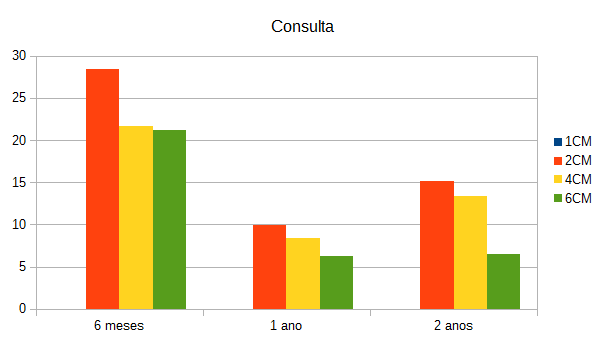
\includegraphics[width=1\textwidth]{figuras/graph_select_buscas.png}
	\caption{Busca de dados}
	\label{fig:graph_select_busca}
\end{figure}

\begin{table}[]
	\centering
	\caption{Busca de dados}
	\label{tab:melhora_select}
	\begin{tabular}{lllll}
		\textbf{Tamanho} & \textbf{1 para 2} & \textbf{2 para 4} & \textbf{4 para 6} & \textbf{Média} \\ \hline
		6 meses          & 40,15\%		 	 & 23,85\%        	 & 2,31\%         	 & 22,10\%        \\ \hline
		1 ano            & 78,99\% 		 	 & 16m47\%       	 & 24,85\%        	 & 40,10\%         \\ \hline
		2 anos           & 91,29\%		 	 & 12,16\%        	 & 50,90\%        	 & 51,45\%         \\ \hline
        Média 		     & 70,14\%		 	 & 17,49\%        	 & 26,02\%        	 & \textbf{30,52}\%         \\ \hline
	\end{tabular}
\end{table}